\newSec[Flight]{Analyse realer Flugdaten}{2}

\newSec[FlightData]{Datenbasis}{3}
Dieses Kapitel zeigt die verschiedenen Daten des Flugs, um diese in der nachfolgenden Analyse einordnen zu können.

Der gezeigte Datensatz enthält zwei Flüge, welche naheinander aufgenommen wurden. Aus diesen Daten wurden irrelevante Einträge zwischen den Flügen entfernt. Durch diesen Eingriff wurde der berechnete Verlauf des zweiten Fluges nicht beeinflusst, da die Status des \Quad[s] zu geeigneten Zeitpunkten zurückgesetzt werden.

Der vom Zustandsautomaten der \Ar\ einnehmbare ZustandIDs sind im \CodePkg{ardrone\_autonomy} wie folgt definiert:
\begin{table}[!ht]
\begin{tabular}{ll}
StatusID & Status-Text    \\ \hline
0        & Unknown        \\
1        & Init           \\
2        & Landed         \\
3        & Flying         \\
4        & Hovering       \\
5        & Test           \\
6        & Taking off     \\
7        & Goto Fix Point \\
8        & Landing        \\
9        & Looping       
\end{tabular}
\end{table}
\FloatBarrier
Aus den Flugversuchen zeigte sich, dass StatusID 6 (\textit{Taking off}) nicht gesendet wird. Stattdessen wird StatusID 7 (\textit{Goto Fix Point}) unmittelbar nach der \textit{Takeoff}-Message eingenommen. StatusID 8 (\textit{Landing}) wird durch StatusID 9 (\textit{Looping}) abgebildet. 


\begin{figure}[ht!]
\vspace{0.25cm}
\begin{center}
\fbox{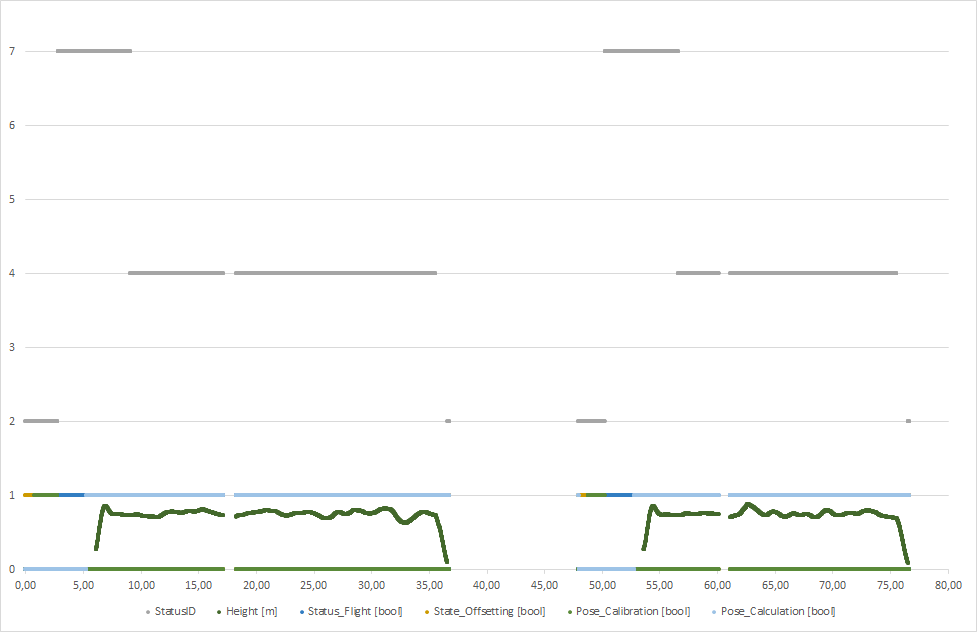
\includegraphics[width=15cm]{Pictures/TestFlight Status Flags Height.png}}
\caption{Testflug: StatusID, Flags und Höhenprofil}
\label{fig:FlightStatus}
\end{center}

\vspace{0.25cm}
Um die Aussagekraft der Graphik zu gewährleisten wurde die Ordinatenachse lediglich bis zum Wert 7 abgebildet. Hierdurch wird die StatusID der Landephase ausgespart.
\end{figure}

Aus den Daten kann eine \textit{ground truth} für die Position der z-Achse entnommen werden. Diese Daten stammen von dem auf den Untergrund gerichteten Ultraschall-Sensor.\\
Eine Genaue Abschätzung der Korrektheit dieser Daten lässt sich nicht aus Vergleichsdaten belegen. Die Genauigkeit des Untraschall-Sensors kann jedoch als höher angenommen werden als die der berechneten Pose.


\FloatBarrier
\newSec[FlightProcess]{Verlauf des Fluges}{3}
Die Flüge in \refImg{fig:FlightStatus} folgen jeweils dem gleichen Scheman:
\begin{enumerate}
\item Der \Quad\ befindet sich in StatusID 2 (\textit{Landed})
\item Die \CodeMeth{reset()} der \CodeClass{IMUable} wird aufgerufen.\\
Dies geschieht mit Initialisierung einer Instanz der \CodeClass{IMUable} oder durch eine User-Eingabe.
\item Die \textit{valid}-Flags der \CodeClass{StateBuildable} und \CodeClass{PoseBuildable} werden zurückgesetzt.
\item Die \CodeClass{StateBuildable} wird in den \textit{Offsetting}-Zustand versetzt.\\
Aus den eingehenden Daten der \textit{IMU}-Nachrichten wird die dauerhaften Nullpunkt-Abweichung geschätzt.
\item In der \CodeClass{PoseBuildable} wird die Kalibrierung eingeleitet. Hierzu werden die eingehenden Instanzen der \CodeClass{IMUState} in einer Liste abgelegt.
\item Aus der User-Eingabe folgt der Start-Befehl.
Die \CodeClass{Statusable} sendet den Befehl an den \Quad\, die StatusID wechselt auf den Wert 7 (\textit{Goto Fix Point}).\\
Die Kalibrierung der \CodeClass{PoseBuildable} wird abgeschlossen: Hierzu werden die in der Liste gespeicherten Werte zur Berechnung einer Pose genutzt. Auf Grund der verstrichenen Zeit kann entsprechend \refCap{ControlPosAccelOffset} die verbliebene dauerhaften Nullpunkt-Abweichung geschätzt werden. Dieser Vorgang wird iterativ durchgeführt.\\
Parallel zur Kalibrierung beginnt der \Quad\ \Ar\ mit dem Start-Vorgang. Dieser sieht vor, die Rotor-Drehzahl zügig zu erhöhen, bis der \Quad\ abhebt und auf eine vom Hersteller vorgegebene Höhe ansteigt.\\
Mit den Erreichen einer empirisch definierten Drehzahl\footnote{Für die \Ar\ ist die Drehzahl in der \CodeClass{parrotIMU} als Konstante \CodeVar{Magic\_TakeoffRotorSpeed} definiert.} wird das \textit{valid}-Flag der \CodeClass{PoseBuilder} gesetzt und ein Rücksetzen der Position ausgelöst.
\item Der Flug endet mit der User-Eingabe des \textit{Landen}-Befehls.\\
Mit dem Erreichen des Wertes 0 für die Rotor-Drehzahl und die Höhe wird das \textit{valid}-Flag der \CodeClass{PoseBuilder} zurückgesetzt.
\end{enumerate}


\newSec[FlightAnalysisLeak]{Lecks der Datenübertragung}{3}
Aus den Daten, aufgetragen in \refImg{fig:FlightStatus}, und weiteren Testflugen zeigt sich, dass die Verbindung zwischen dem Host-PC und dem \Quad\ anfällig für Verbindungsunterbrechnungen ist. Während diesen Unterbrechnungen werden für einen Zeitraum von etwa einer Sekunde keine Nachrichten übermittelt.\\
Die entwickelte Software sieht für diese Fälle keine Interpolation der Daten vor. Hieraus entstehen Sprünge in den berechneten Daten und durch die Integration dieser veränderten Daten ein Drift der Position. Hier können als Beispiel \refImg{fig:FlightPoseVel} und \refImg{fig:FlightPos} jeweils für die Zeitbereiche um 17 Sekunden und 61 Sekunden herangezogen werden.







